\documentclass[a4paper,11pt]{article}

\usepackage{inputenc}
\usepackage[T1]{fontenc}
\usepackage[frenchb]{babel}
\usepackage{fancyhdr,fancybox} % pour personnaliser les en-têtes
\usepackage{lastpage,setspace}
\usepackage{amsfonts,amssymb,amsmath,amsthm,mathrsfs}
\usepackage{mathdots}
\usepackage{relsize,exscale,bbold}
\usepackage{paralist}
\usepackage{xspace,multicol,diagbox,array}
\usepackage{xcolor}
\usepackage{variations}
\usepackage{xypic}
\usepackage{eurosym,stmaryrd}
\usepackage{graphicx}
\usepackage[np]{numprint}
\usepackage{hyperref} 
\usepackage{tikz}
\usepackage{colortbl}
\usepackage{multirow}
\usepackage{MnSymbol,wasysym}
\usepackage[top=1.5cm,bottom=1.5cm,right=1.2cm,left=0.05cm]{geometry}
\usetikzlibrary{calc, arrows, plotmarks, babel,decorations.pathreplacing}


\begin{document}
	

	
	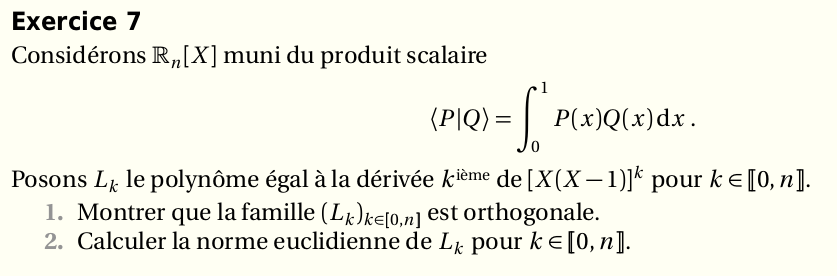
\includegraphics[scale=0.5]{c1.png}

	

	
	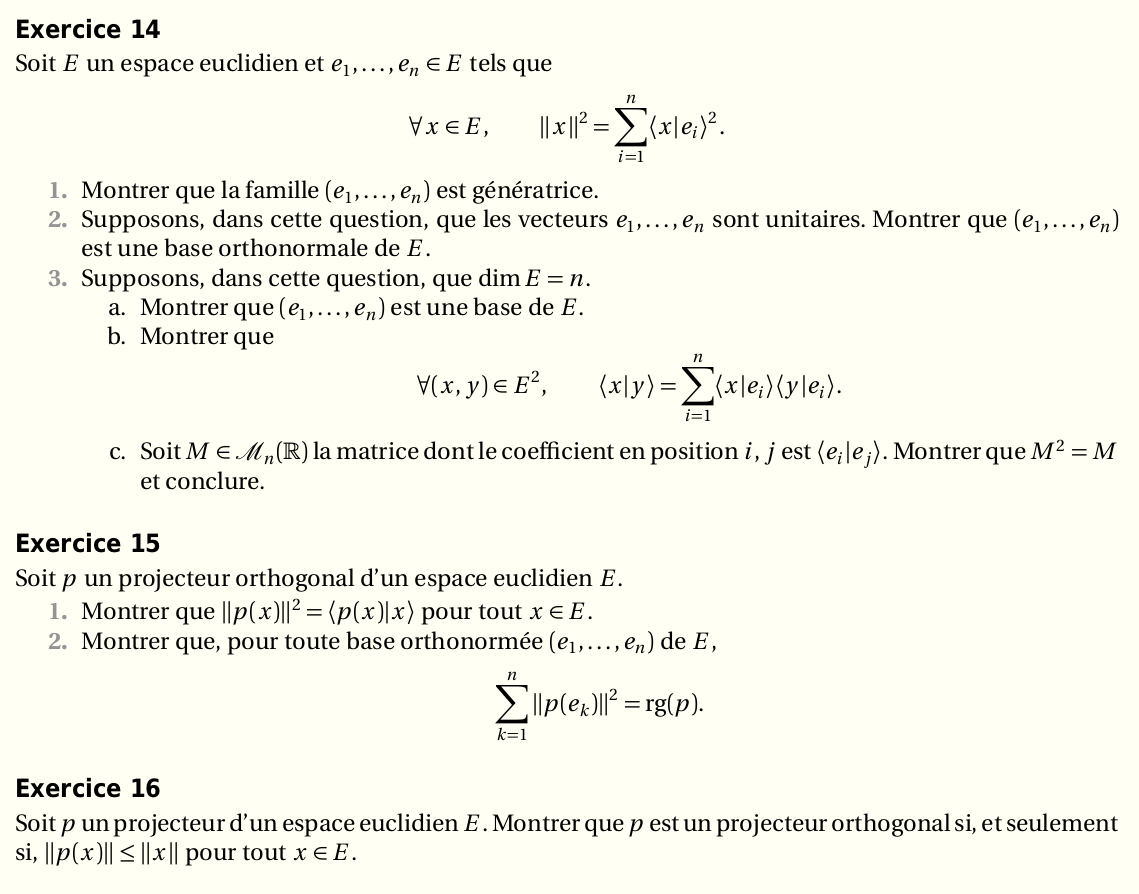
\includegraphics[scale=0.5]{c2.png}
	

\end{document}
